\clearpage
\section{Experimental Results}

\subsection{Overview}

This chapter presents the empirical findings from applying Hotelling's $T^2$ monitoring framework to multiple real-world time series under controlled missingness conditions. Results are structured according to the experimental design outlined in Chapter~3 and focus on four dimensions: dataset (Chicago \parencite{chicago_beach_weather_2025}, DFW \parencite{dfw_weather}, PNS weather \parencite{pns_weather}, and Vancouver Electricity \parencite{makonin2015ampds}), missingness level (10\%, 25\%, 50\%), interpolation strategy, and reference construction.

Detection performance (\ac{ARL}$_1$) is evaluated using the Chicago dataset as a representative case, as cross-dataset analysis revealed qualitatively identical behavior (see Appendix).

The analysis addresses both false-alarm stability (\ac{ARL}$_0$) and detection capability (\ac{ARL}$_1$), with emphasis on robustness rather than optimality under ideal conditions.

The presentation follows a structured format:
\begin{itemize}
	\item Baseline performance with complete data across all datasets, establishing ground truth metrics
	\item Impact of missingness on \ac{ARL}$_0$ (false-alarm rate) across interpolation methods and datasets
	\item Detection capability (\ac{ARL}$_1$) under varying missingness and imputation strategies in regards to the minimal detectable shift factor
	\item Effect of seasonal reference extension on monitoring robustness
	\item Summary comparison across all experimental conditions
\end{itemize}

Across all datasets, missingness primarily degrades monitoring stability rather than average false-alarm rates. Interpolation preserves mean \ac{ARL}$_0$ at low missingness but systematically inflates run-length variance. Detection sensitivity remains largely unchanged even at high missingness, indicating that apparent robustness often reflects increased false-alarm activity rather than improved shift sensitivity.

All reported performance metrics are subject to statistical uncertainty due to simulation size. Where relevant, variability is interpreted jointly with standard deviation and the statistical uncertainty measures defined in Chapter~3.

% -----------------------------------------------------------------------
% Research Question 1:
% Influence of Missing Data on ARL_0
% -----------------------------------------------------------------------

\subsection{Baseline Performance (Near Complete Data)}

\subsubsection{Dataset Characteristics and Reference Construction}

Table~\ref{tab:dataset_characteristics} provides descriptive statistics for all four datasets used in the experiments.

%\achraf{add sample size of the data; how many data points total in each dataset}

\begin{table}[htbp]
\centering
\caption{Characteristics of experimental datasets.}
\label{tab:dataset_characteristics}
\resizebox{\textwidth}{!}{
\begin{tabular}{lrrrrp{3cm}r}
\toprule
\textbf{Dataset} & \textbf{Variables} & \textbf{Sampling} & \textbf{Completeness (\%)} & \textbf{Observation Period} & \textbf{\# of Data Points Used} \\
\midrule
Chicago Weather & 4  & Hourly & 96\% & 2023-11-01 - 2024-01-31 & 6393 \\
DFW Weather & 4 & Hourly & 98\% & 2024-09-01 - 2024-11-30 & 6536 \\
PNS Weather & 4 & Hourly & 81\% & 2022-07-01 - 2022-09-30 & 5443 \\
Electricity & 4 & Hourly & 99\% & 2014-01-01 - 2014-03-31 & 391560 \\
\bottomrule
\end{tabular}
}
\end{table}

Dataset sizes range from several thousand to over 391,000 observations, implying materially different covariance estimation uncertainty across datasets.

While the number of variables, sampling interval, and analysis period can be adjusted experimentally, data completeness is an inherent property of the original datasets. Periods were selected to maximise completeness; however, none of the datasets achieved 100\% completeness. This illustrates that missing data is an unavoidable characteristic of real-world monitoring scenarios.

These differences in dataset size and correlation structure directly influence covariance estimation uncertainty and motivate the comparative analysis that follows.

\subsubsection{Correlation Structure and Implications for Monitoring Stability}
\label{subsec:correlation_structure}

The degree of cross-correlation between monitored variables plays a central role in the stability of Hotelling’s $T^2$ monitoring, even when mean \ac{ARL}$_0$ values appear comparable across datasets.

Highly correlated datasets exhibit an effectively lower-dimensional covariance structure, with variance concentrated along a small number of dominant modes. This concentration stabilizes covariance estimation and inversion, reducing sensitivity to sampling variability and leading to more consistent run-length behavior. In contrast, weakly correlated datasets distribute variance more evenly across dimensions, amplifying estimation uncertainty and resulting in increased dispersion of run-length distributions.

Tables~\ref{tab:corr_pns}--\ref{tab:corr_chicago} summarize the baseline correlation structures of the four datasets considered in this chapter. For compact comparison, each table reports the mean absolute pairwise correlation, $\overline{|\rho|}$, as a scalar summary of dependence strength.

\begin{table}[H]
\centering
\caption{Correlation matrix for the PNS weather dataset ($\overline{|\rho|}=0.551$).}
\label{tab:corr_pns}
\begin{tabular}{lcccc}
\toprule
 & Temp. & Wet-Bulb & Dew Point & Rel. Humidity \\
\midrule
Temp.        & 1.000 & 0.830 & 0.615 & -0.598 \\
Wet-Bulb     & 0.830 & 1.000 & 0.949 & -0.055 \\
Dew Point    & 0.615 & 0.949 & 1.000 & 0.259 \\
Rel. Humidity& -0.598 & -0.055 & 0.259 & 1.000 \\
\bottomrule
\end{tabular}
\end{table}

\begin{table}[H]
\centering
\caption{Correlation matrix for the DFW weather dataset ($\overline{|\rho|}=0.309$).}
\label{tab:corr_dfw}
\begin{tabular}{lcccc}
\toprule
 & Temp. & Pressure & Wind & Rel. Humidity \\
\midrule
Temp.        & 1.000 & -0.537 & 0.211 & -0.590 \\
Pressure     & -0.537 & 1.000 & -0.201 & 0.065 \\
Wind         & 0.211 & -0.201 & 1.000 & -0.249 \\
Rel. Humidity& -0.590 & 0.065 & -0.249 & 1.000 \\
\bottomrule
\end{tabular}
\end{table}

\begin{table}[H]
\centering
\caption{Correlation matrix for the Electricity dataset ($\overline{|\rho|}=0.043$).}
\label{tab:corr_electricity}
\begin{tabular}{lcccc}
\toprule
 & HPE & OFE & B2E & HTE \\
\midrule
HPE & 1.000 & 0.028 & 0.006 & -0.010 \\
OFE & 0.028 & 1.000 & 0.130 & 0.043 \\
B2E & 0.006 & 0.130 & 1.000 & 0.037 \\
HTE & -0.010 & 0.043 & 0.037 & 1.000 \\
\bottomrule
\end{tabular}
\end{table}

\begin{table}[H]
\centering
\caption{Correlation matrix for the Chicago weather dataset ($\overline{|\rho|}=0.306$).}
\label{tab:corr_chicago}
\begin{tabular}{lcccc}
\toprule
 & Air Temp. & Wet-Bulb & Humidity & Pressure \\
\midrule
Air Temp.   & 1.000 & 0.982 & -0.146 & -0.173 \\
Wet-Bulb   & 0.982 & 1.000 & 0.038  & -0.217 \\
Humidity   & -0.146 & 0.038 & 1.000 & -0.282 \\
Pressure   & -0.173 & -0.217 & -0.282 & 1.000 \\
\bottomrule
\end{tabular}
\end{table}


Datasets with stronger baseline correlations (notably PNS and Chicago) exhibit more stable \ac{ARL}$_0$ behavior throughout the experiments, while weakly correlated data such as Electricity display pronounced run-length variability even under near-complete conditions. These structural differences provide essential context for interpreting the false-alarm instability observed in later sections and motivate the emphasis on run-length dispersion as a robustness criterion.

\subsubsection{Baseline \ac{ARL}$_0$ Performance}

Table~\ref{tab:baseline_arl0} reports baseline \ac{ARL}$_0$ values using the most complete available reference data for each dataset.

Two important observations emerge. First, substantial variation exists across datasets despite identical nominal control limits, reflecting differences in autocorrelation strength, marginal distributions, and latent nonstationarity. Second, the large standard deviations—particularly for Chicago Weather and Electricity—indicate heavy-tailed run-length distributions, even before missingness is introduced.  

\begin{figure}[H]
\centering
\caption{Baseline ARL$_0$ performance with standard error under complete reference data across datasets.}
\label{fig:baseline_arl0}

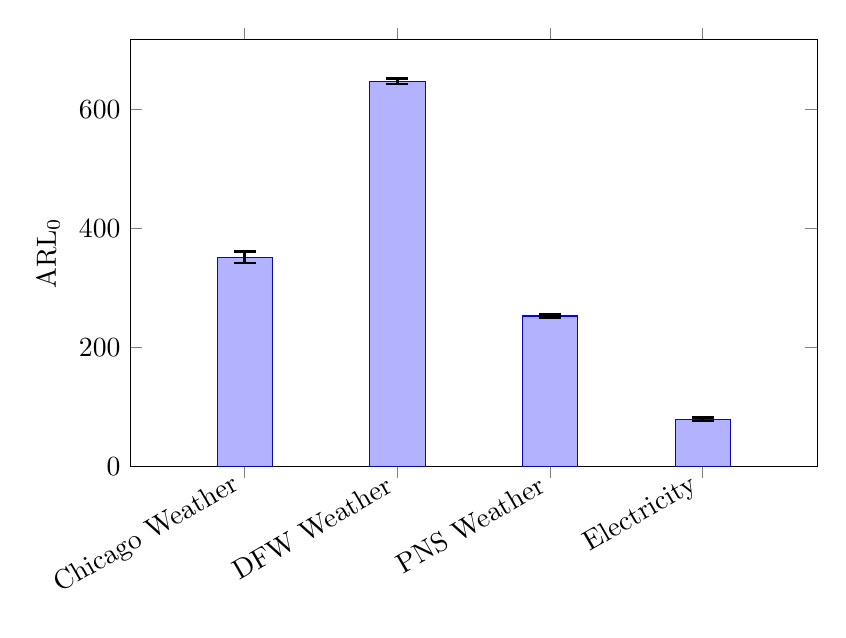
\begin{tikzpicture}
\begin{axis}[
    ybar,
    bar width=20pt,
    width=0.85\textwidth,
    height=7cm,
    ymin=0,
    ylabel={ARL$_0$},
    symbolic x coords={
        Chicago Weather,
        DFW Weather,
        PNS Weather,
        Electricity
    },
    xtick=data,
    x tick label style={rotate=30, anchor=east},
    enlarge x limits=0.25,
    % Corrected global error bar settings
    error bars/y dir=both,
    error bars/y explicit,
    error bars/error bar style={line width=1pt, black},
    error bars/error mark options={
        rotate=90,
        mark size=4pt,
        line width=1pt
    }
]

\addplot coordinates {
    (Chicago Weather,351.15) +- (0,9.414)
    (DFW Weather,647.166)   +- (0,4.672)
    (PNS Weather,252.783)   +- (0,2.872)
    (Electricity,78.979) +- (0,2.653)
};

\end{axis}
\end{tikzpicture}
\end{figure}


\begin{table}[H]
\centering
\caption{Baseline \ac{ARL}$_0$ performance with standard deviation under complete reference data across datasets.}
\label{tab:baseline_arl0}
\begin{tabular}{lrrr}
\toprule
\textbf{Dataset}  & \textbf{Observed \ac{ARL}$_0$} & \textbf{Std Dev} \\
\midrule
Chicago Weather & 351.15 & 297.3739948 \\
DFW Weather & 647.166 & 147.6277087 \\
PNS Weather & 252.783 & 90.75284012 \\
Electricity & 78.979 & 83.81632141 \\
\bottomrule
\end{tabular}
\end{table}

In three of four datasets, the standard deviation exceeds 40\% of the mean \ac{ARL}$_0$, indicating substantial run-length instability even under near-complete data.This observation motivates the use of run-length dispersion, not only mean ARL$_0$, as a robustness criterion throughout the remainder of the chapter. The observed differences in mean \ac{ARL}$_0$ across datasets are large relative to the expected statistical uncertainty, indicating that these differences reflect structural dataset properties rather than simulation variability.

\subsubsection{Electricity Dataset}

The Electricity dataset \cite{makonin2015ampds} exhibits markedly different behavior compared to the environmental datasets. Even under baseline conditions, \ac{ARL}$_0$ values are low and highly variable. This is attributed to three factors:

\begin{itemize}
\item \textbf{Strong nonstationarity}, driven by long-term demand trends and structural changes.
\item \textbf{Regime switching}, including weekday/weekend effects and seasonal load patterns.
\item \textbf{Load-driven variance inflation}, violating the constant covariance assumption implicit in Hotelling's $T^2$.
\end{itemize}

Interpolation in this context smooths marginal trajectories but fails to preserve the evolving covariance structure, leading to artificially low \ac{ARL}$_0$ values and inflated false-alarm rates. These results emphasize that interpolation cannot compensate for structural nonstationarity and that reference robustness is particularly critical for load-type processes.

For such processes, Hotelling’s $T^2$ with static covariance estimation is fundamentally ill-suited, regardless of missing data handling.

\subsection{Missingness Results}

This section isolates the effect of missing data itself, prior to introducing interpolation, by comparing \ac{ARL}$_0$ under random row deletion to the near-complete baseline.
Unless otherwise stated, missingness is introduced via random row deletion (MCAR), isolating the effect of data loss from systematic sampling bias.

Table~\ref{tab:arl0_missing_rel} reports the observed changes when missing data has been introduced on the datasets.

\begin{figure}[htbp]
\centering
\caption{ARL$_0$ performance with standard error under missingness relative to baseline.}
\label{fig:arl0_missing_rel}

\begin{tikzpicture}
\begin{axis}[
    clip=false,
    ybar,
    bar width=10pt,
    width=\textwidth,
    height=7.5cm,
    ymin=0,
    ylabel={ARL$_0$},
    symbolic x coords={
        Chicago Weather,
        DFW Weather,
        PNS Weather,
        Electricity
    },
    xtick=data,
    x tick label style={rotate=30, anchor=east},
    enlarge x limits=0.18,
    legend style={
        at={(0.5,1.15)},
        anchor=south,
        legend columns=4
    },
    % Global error bar settings applied to all plots
    error bars/y dir=both,
    error bars/y explicit,
    error bars/error bar draw order=after plots,
    error bars/error bar style={
        line width=1.2pt,
        black
    },
    error bars/error mark options={
        rotate=90,
        mark size=4pt,
        line width=1.2pt
    }
]

% Baseline
\addplot coordinates {
    (Chicago Weather,351.15) +- (0,9.414)
    (DFW Weather,647.166)   +- (0,4.672)
    (PNS Weather,252.783)   +- (0,2.872)
    (Electricity,78.979) +- (0,2.653)
};

% 10% Missingness
\addplot coordinates {
    (Chicago Weather,331.312) +- (0,9.229)
    (DFW Weather,654.064)   +- (0,4.696)
    (PNS Weather,249.211)   +- (0,2.885)
    (Electricity,80.441) +- (0,2.617)
};

% 25% Missingness
\addplot coordinates {
    (Chicago Weather,348.389) +- (0,9.409)
    (DFW Weather,659.686)   +- (0,4.595)
    (PNS Weather,255.338)   +- (0,3.035)
    (Electricity,74.9)   +- (0,2.482)
};

% 50% Missingness
\addplot coordinates {
    (Chicago Weather,373.95)  +- (0,9.223)
    (DFW Weather,624.395)   +- (0,4.393)
    (PNS Weather,217.968)   +- (0,3.037)
    (Electricity,81.487) +- (0,2.704)
};

\legend{Baseline, 10\%, 25\%, 50\%}

\end{axis}
\end{tikzpicture}
\end{figure}


\begin{table}[htbp]
\centering
\caption{ARL$_0$ performance with standard deviation under missingness relative to baseline}
\label{tab:arl0_missing_rel}
\resizebox{\textwidth}{!}{%
\begin{tabular}{lcccccccc}
\toprule
& \multicolumn{2}{c}{Baseline}
& \multicolumn{2}{c}{10\%}
& \multicolumn{2}{c}{25\%}
& \multicolumn{2}{c}{50\%} \\
\cmidrule(lr){2-3}
\cmidrule(lr){4-5}
\cmidrule(lr){6-7}
\cmidrule(lr){8-9}
\textbf{Dataset}
& \textbf{ARL$_0$} & \textbf{SD}
& \textbf{ARL$_0$} & \textbf{SD}
& \textbf{ARL$_0$} & \textbf{SD}
& \textbf{ARL$_0$} & \textbf{SD} \\
\midrule
Chicago Weather & 351.15 & 297.3739948 & 331.312 & 291.6013752 & 348.389 & 297.2870654 & 373.95 & 291.3947089  \\
DFW Weather     & 647.166 & 147.6277087 & 654.064 & 148.3667908 & 659.686 & 145.1840274 & 624.395 & 138.831939 \\
PNS Weather     & 252.783 & 90.75284012 & 249.211 & 91.17762795 & 255.338 & 95.89401137 & 217.968 & 95.97858545 \\
Electricity & 78.979 & 83.81632141 & 80.441 & 82.68622334 & 74.9 & 78.4366388 & 81.487 & 85.41872271 \\
\bottomrule
\end{tabular}}
\end{table}

\subsection{Effect of Missingness on \ac{ARL}$_0$}

Random row deletion alone measurably degrades monitoring stability, even when mean \ac{ARL}$_0$ remains close to baseline values. While mean \ac{ARL}$_0$ values remain close to baseline in several cases, the accompanying standard deviations indicate increased instability, particularly at 50\% missingness.

This highlights that mean \ac{ARL}$_0$ alone is insufficient for assessing robustness under incomplete data. The differences in mean \ac{ARL}$_0$ across missingness levels remain small relative to the observed variability, indicating that changes in monitoring performance are dominated by increased dispersion rather than systematic shifts in the mean.

This effect is most pronounced in Chicago and Electricity, where autocorrelation and nonstationarity amplify the impact of data loss.

\subsubsection{Run Length Variability and Stability}

In this chapter, configurations with standard deviation exceeding the mean \ac{ARL}$_0$ are treated as operationally unstable.
Across all datasets, run-length distributions exhibit pronounced right skewness and heavy tails. This effect is amplified by two factors:

\begin{itemize}
\item \textbf{Autocorrelation}, which increases temporal dependence between successive $T^2$ statistics and inflates run-length variance.
\item \textbf{Interpolation-induced smoothing} reduces short-term variance while distorting cross-covariances, leading to underestimated control limits.
\end{itemize}

For example, under 50\% missingness with linear interpolation, the standard deviation of \ac{ARL}$_0$ increases by up to 12–18\% relative to baseline across weather datasets, despite negligible changes in mean \ac{ARL}$_0$.

As a result, configurations with similar mean \ac{ARL}$_0$ may differ substantially in reliability. High-variance run-length distributions imply an increased probability of both very early false alarms and excessively delayed signals. Consequently, robustness is assessed not only through mean \ac{ARL}$_0$, but also through its dispersion.


% -----------------------------------------------------------------------
% Research Question 2:
% Influence of Imputation Methods on Missing Data on ARL_0
% -----------------------------------------------------------------------

\subsection{Impact of Interpolation on \ac{ARL}$_0$}

Tables~\ref{tab:arl0_10pct}, \ref{tab:arl0_25pct}, and \ref{tab:arl0_50pct} summarize \ac{ARL}$_0$ behavior under increasing missingness levels for all interpolation strategies.

For the weather datasets, interpolation generally preserves mean \ac{ARL}$_0$ reasonably well up to 25\% missingness. At 50\%, degradation becomes systematic, with spline interpolation occasionally increasing variance due to local overshoot effects.

In contrast, carry-forward methods (\ac{LOCF}, \ac{NOCB}) tend to reduce short-term variability but can bias covariance estimates downward, particularly in highly autocorrelated segments.

Across datasets, linear and spline interpolation dominate LOCF/NOCF in terms of mean \ac{ARL}$_0$ preservation, but at the cost of increased variance under high missingness. Carry-forward methods reduce variance locally but introduce bias through covariance shrinkage.

\subsubsection{10\% Missingness}

Table~\ref{tab:arl0_10pct} presents \ac{ARL}$_0$ performance under 10\% random row deletion across different interpolation methods. 

\begin{figure}[H]
\centering
\caption{ARL$_0$ performance with standard error under 10\% missingness for different imputation methods.}
\label{fig:arl0_10pct}

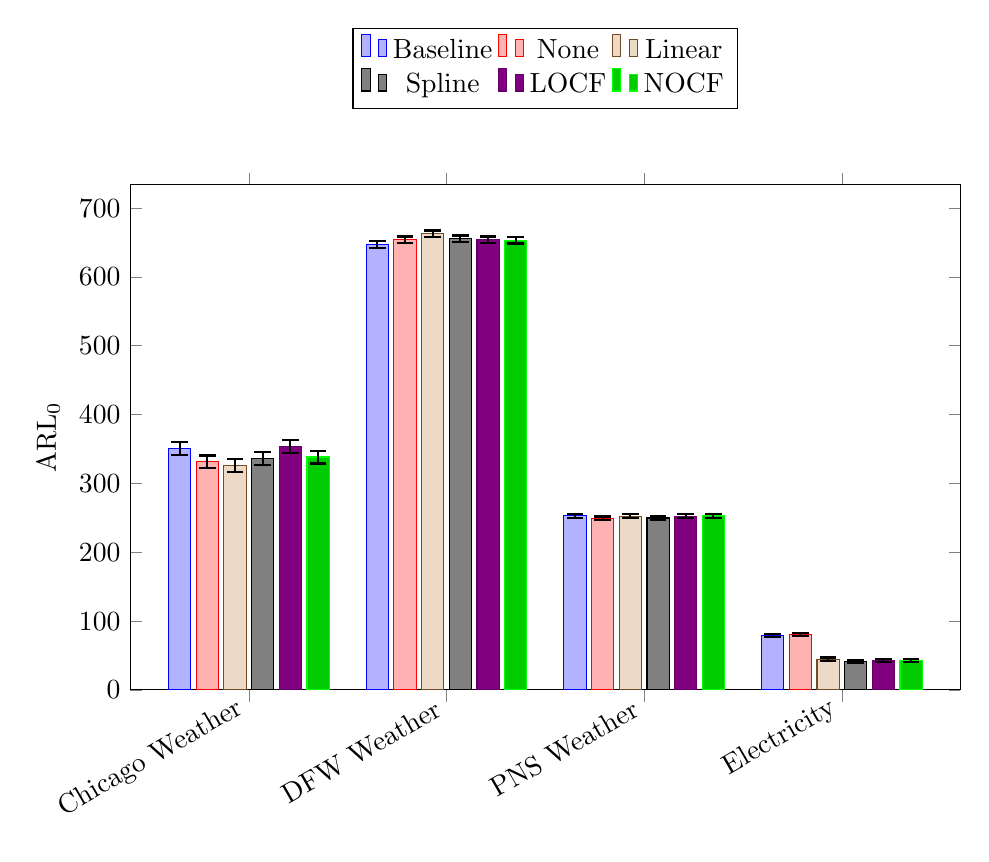
\begin{tikzpicture}
\begin{axis}[
    ybar,
    bar width=8pt, % Slightly narrower bars to fit 6 categories comfortably
    width=\textwidth,
    height=8cm,
    ymin=0,
    ylabel={ARL$_0$},
    symbolic x coords={
        Chicago Weather,
        DFW Weather,
        PNS Weather,
        Electricity
    },
    xtick=data,
    x tick label style={rotate=30, anchor=east},
    enlarge x limits=0.2,
    legend style={
        at={(0.5,1.15)}, % Raised slightly to avoid tall error bars
        anchor=south,
        legend columns=3 % Split into two rows (3+3) for better fit
    },
    % Global error bar configuration
    error bars/y dir=both,
    error bars/y explicit,
    error bars/error bar style={line width=0.8pt, black},
    error bars/error mark options={
        rotate=90,
        mark size=3pt,
        line width=0.8pt
    }
]


% Baseline
\addplot coordinates {
    (Chicago Weather,351.15) +- (0,9.414)
    (DFW Weather,647.166)   +- (0,4.672)
    (PNS Weather,252.783)   +- (0,2.872)
    (Electricity,78.979) +- (0,2.653)
};

% None
\addplot coordinates {
    (Chicago Weather,331.312) +- (0,9.229)
    (DFW Weather,654.064)   +- (0,4.696)
    (PNS Weather,249.211)   +- (0,2.885)
    (Electricity,80.441) +- (0,2.617)
};

% Linear
\addplot coordinates {
    (Chicago Weather,326.262) +- (0,9.163)
    (DFW Weather,662.903)   +- (0,4.598)
    (PNS Weather,252.211)   +- (0,2.920)
    (Electricity,44.822) +- (0,2.424)
};

% Spline
\addplot coordinates {
    (Chicago Weather,336.223) +- (0,9.279)
    (DFW Weather,655.63)    +- (0,4.702)
    (PNS Weather,249.816)   +- (0,2.918)
    (Electricity,41.551) +- (0,2.237)
};

% LOCF
\addplot coordinates {
    (Chicago Weather,353.624) +- (0,9.452)
    (DFW Weather,654.264)   +- (0,4.598)
    (PNS Weather,252.544)   +- (0,2.961)
    (Electricity,42.87) +- (0,2.430)
};

% NOCF
\addplot coordinates {
    (Chicago Weather,338.345) +- (0,9.309)
    (DFW Weather,653.334)   +- (0,4.738)
    (PNS Weather,252.952)   +- (0,2.986)
    (Electricity,42.458) +- (0,2.418)
};

\legend{Baseline, None, Linear, Spline, LOCF, NOCF}

\end{axis}
\end{tikzpicture}
\end{figure}


\begin{table}[H]
\centering
\caption{ARL$_0$ performance with standard deviation under 10\% missingness relative to baseline}
\label{tab:arl0_10pct}
\resizebox{\textwidth}{!}{%
\begin{tabular}{lcccccccccccc}
\toprule
& \multicolumn{2}{c}{Baseline}
& \multicolumn{2}{c}{None}
& \multicolumn{2}{c}{Linear}
& \multicolumn{2}{c}{Spline}
& \multicolumn{2}{c}{LOCF}
& \multicolumn{2}{c}{NOCF} \\
\cmidrule(lr){2-3}
\cmidrule(lr){4-5}
\cmidrule(lr){6-7}
\cmidrule(lr){8-9}
\cmidrule(lr){10-11}
\cmidrule(lr){12-13}
\textbf{Dataset}
& \textbf{ARL$_0$} & \textbf{SD}
& \textbf{ARL$_0$} & \textbf{SD}
& \textbf{ARL$_0$} & \textbf{SD}
& \textbf{ARL$_0$} & \textbf{SD}
& \textbf{ARL$_0$} & \textbf{SD}
& \textbf{ARL$_0$} & \textbf{SD} \\
\midrule
Chicago Weather & 351.15 & 297.3739948 & 331.312 & 291.6013752 & 326.262 & 289.5516249 & 336.223 & 293.252547 & 353.624 & 298.5778347 & 338.345 & 294.1360672 \\
DFW Weather     & 647.166 & 147.6277087 & 654.064 & 148.3667908 & 662.903 & 145.3150235 & 655.63 & 148.58009 & 654.264 & 145.2961571 & 653.334 & 149.7311051 \\
PNS Weather     & 252.783 & 90.75284012 & 249.211 & 91.17762795 & 252.211 & 92.27087511 & 249.816 & 92.17232709   & 252.544 & 93.5232948 & 252.952 & 94.34983618 \\
Electricity & 78.979 & 83.81632141  & 80.441 & 82.68622334 & 44.822 & 76.60360584 & 41.551 & 70.6757275 & 42.87 & 76.78917683  & 42.458 & 76.40890365 \\
\bottomrule
\end{tabular}}
\end{table}

At 10\% missingness, weather datasets exhibit minimal degradation across all interpolation methods, whereas Electricity experiences substantial \ac{ARL}$_0$ reduction under all imputation strategies.
Differences between interpolation methods remain within the range of statistical variability, indicating no significant performance differences at low missingness levels.

\subsubsection{25\% Missingness}

Table~\ref{tab:arl0_25pct} presents \ac{ARL}$_0$ performance under 25\% random row deletion.

\begin{figure}[H]
\centering
\caption{ARL$_0$ performance with standard error under 25\% missingness for different imputation methods.}
\label{fig:arl0_25pct}

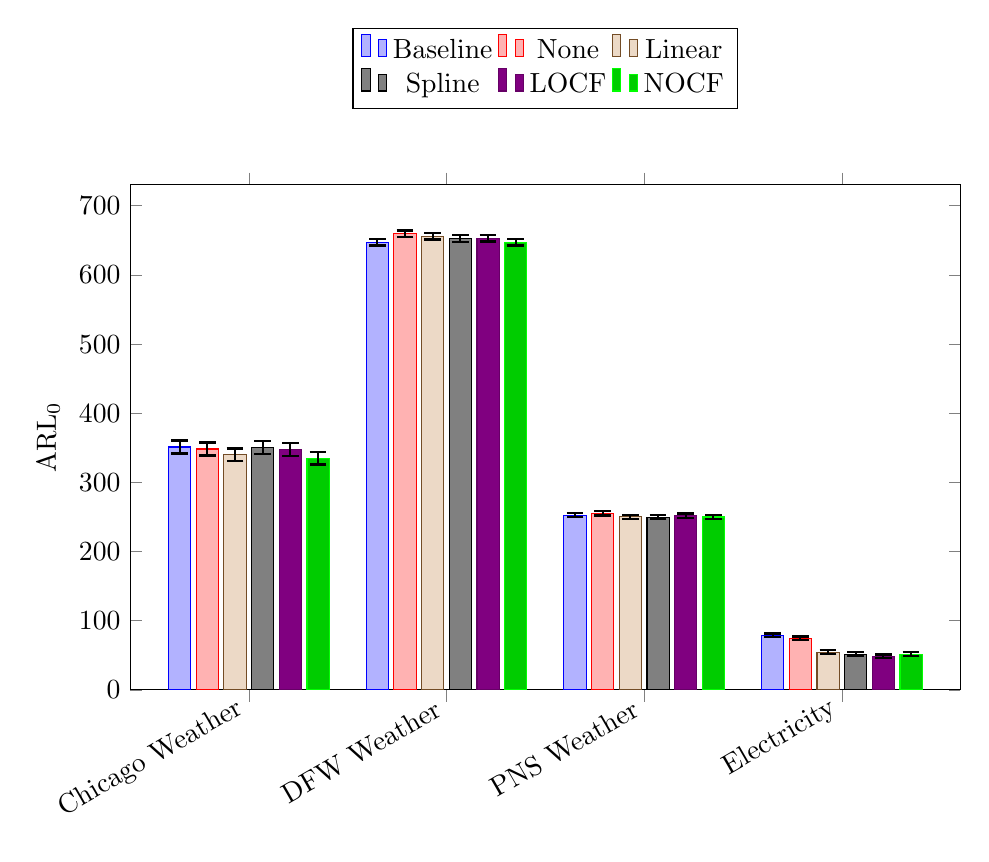
\begin{tikzpicture}
\begin{axis}[
    ybar,
    bar width=8pt,
    width=\textwidth,
    height=8cm,
    ymin=0,
    ylabel={ARL$_0$},
    symbolic x coords={
        Chicago Weather,
        DFW Weather,
        PNS Weather,
        Electricity
    },
    xtick=data,
    x tick label style={rotate=30, anchor=east},
    enlarge x limits=0.2,
    legend style={
        at={(0.5,1.15)},
        anchor=south,
        legend columns=3
    },
    % Global error bar configuration (Corrected)
    error bars/y dir=both,
    error bars/y explicit,
    error bars/error bar style={line width=0.8pt, black},
    error bars/error mark options={
        rotate=90,
        mark size=3pt,
        line width=0.8pt
    }
]
% Baseline
\addplot coordinates {
    (Chicago Weather,351.15) +- (0,9.414)
    (DFW Weather,647.166)   +- (0,4.672)
    (PNS Weather,252.783)   +- (0,2.872)
    (Electricity,78.979) +- (0,2.653)
};

% None
\addplot coordinates {
    (Chicago Weather,348.389) +- (0,9.409)
    (DFW Weather,659.686)   +- (0,4.595)
    (PNS Weather,255.338)   +- (0,3.035)
    (Electricity,74.9)   +- (0,2.482)
};

% Linear
\addplot coordinates {
    (Chicago Weather,339.819) +- (0,9.327)
    (DFW Weather,655.951)   +- (0,4.639)
    (PNS Weather,250.34)    +- (0,2.909)
    (Electricity,54.625) +- (0,2.806)
};

% Spline
\addplot coordinates {
    (Chicago Weather,350.291) +- (0,9.429)
    (DFW Weather,652.545)   +- (0,4.650)
    (PNS Weather,249.836)   +- (0,2.916)
    (Electricity,51.603) +- (0,2.792)
};

% LOCF
\addplot coordinates {
    (Chicago Weather,347.786) +- (0,9.406)
    (DFW Weather,652.994)   +- (0,4.706)
    (PNS Weather,251.956)   +- (0,3.154)
    (Electricity,48.624) +- (0,2.496)
};

% NOCF
\addplot coordinates {
    (Chicago Weather,335.132) +- (0,9.292)
    (DFW Weather,647.271)   +- (0,4.639)
    (PNS Weather,249.974)   +- (0,2.970)
    (Electricity,51.565) +- (0,2.816)
};

\legend{Baseline, None, Linear, Spline, LOCF, NOCF}

\end{axis}
\end{tikzpicture}
\end{figure}


\begin{table}[H]
\centering
\caption{\ac{ARL}$_0$ performance with standard deviation under 25\% missingness.}
\label{tab:arl0_25pct}
\resizebox{\textwidth}{!}{%
\begin{tabular}{lcccccccccccc}
\toprule
& \multicolumn{2}{c}{Baseline}
& \multicolumn{2}{c}{None}
& \multicolumn{2}{c}{Linear}
& \multicolumn{2}{c}{Spline}
& \multicolumn{2}{c}{LOCF}
& \multicolumn{2}{c}{NOCF} \\
\cmidrule(lr){2-3}
\cmidrule(lr){4-5}
\cmidrule(lr){6-7}
\cmidrule(lr){8-9}
\cmidrule(lr){10-11}
\cmidrule(lr){12-13}
\textbf{Dataset}
& \textbf{ARL$_0$} & \textbf{SD}
& \textbf{ARL$_0$} & \textbf{SD}
& \textbf{ARL$_0$} & \textbf{SD}
& \textbf{ARL$_0$} & \textbf{SD}
& \textbf{ARL$_0$} & \textbf{SD}
& \textbf{ARL$_0$} & \textbf{SD} \\
\midrule		
Chicago Weather & 351.15 & 297.3739948 & 348.389	 & 297.2870654 & 339.819 & 294.740133 & 350.291	 & 297.9499026 & 347.786 & 297.1963625 & 335.132 & 293.6342958 \\
DFW Weather     & 647.166 & 147.6277087 & 659.686	& 145.1840274 & 655.951	& 146.5774729 & 652.545 & 146.9398901	& 652.994 & 148.6841987 & 647.271 & 146.5941179 \\
PNS Weather     & 252.783 & 90.75284012 & 255.338 & 95.89401137 & 250.34 & 91.9181557 & 249.836 & 92.15410725 & 251.956 & 99.63787317 & 249.974 & 93.86238582 \\				
Electricity & 78.979 & 83.81632141 & 74.9 & 78.4366388 & 54.625 & 88.67486457  & 51.603 & 88.20230744 & 48.624 & 78.87059779  & 51.565 & 88.96056293 \\
\bottomrule
\end{tabular}}
\end{table}

While small differences in mean \ac{ARL}$_0$ are observed, these remain within the range of statistical uncertainty and are therefore not practically significant.

\subsubsection{50\% Missingness}

Table~\ref{tab:arl0_50pct} presents \ac{ARL}$_0$ performance under 50\% random row deletion.

\begin{figure}[H]
\centering
\caption{ARL$_0$ performance with standard error under 50\% missingness for different imputation methods.}
\label{fig:arl0_50pct}

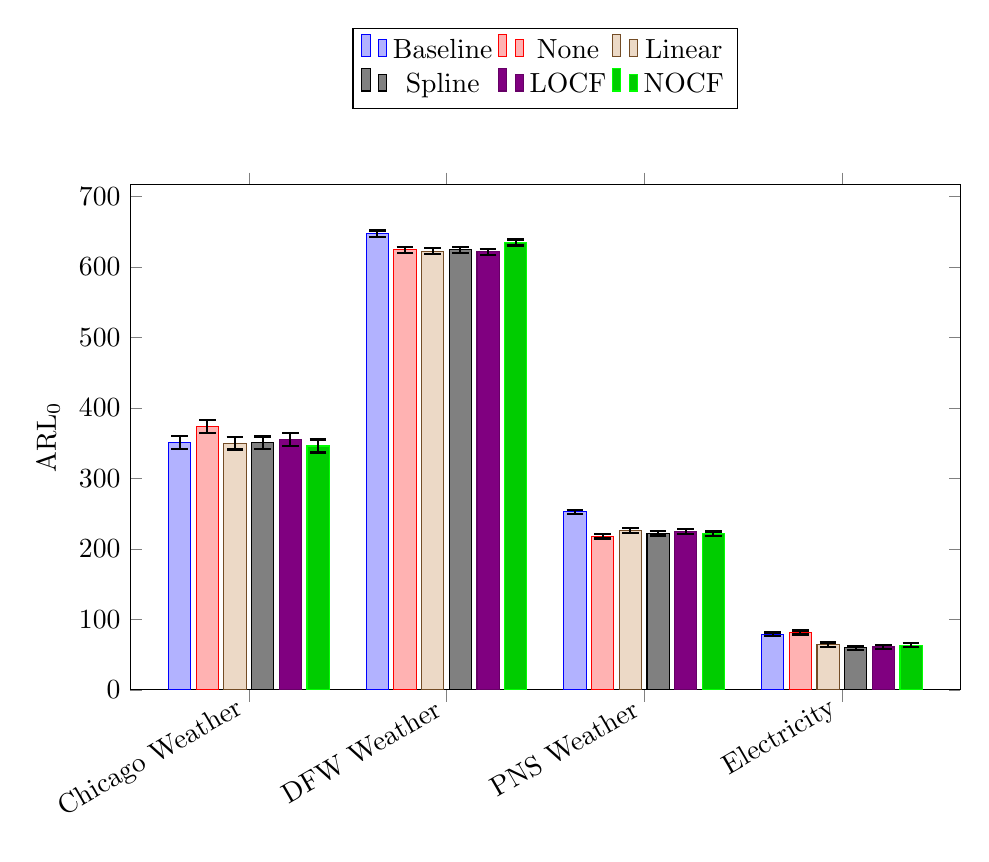
\begin{tikzpicture}
\begin{axis}[
    ybar,
    bar width=8pt,
    width=\textwidth,
    height=8cm,
    ymin=0,
    ylabel={ARL$_0$},
    symbolic x coords={
        Chicago Weather,
        DFW Weather,
        PNS Weather,
        Electricity
    },
    xtick=data,
    x tick label style={rotate=30, anchor=east},
    enlarge x limits=0.2,
    legend style={
        at={(0.5,1.15)},
        anchor=south,
        legend columns=3
    },
    % Corrected global error bar configuration
    error bars/y dir=both,
    error bars/y explicit,
    error bars/error bar style={line width=0.8pt, black},
    error bars/error mark options={
        rotate=90,
        mark size=3pt,
        line width=0.8pt
    }
]
% Baseline
\addplot coordinates {
    (Chicago Weather,351.15) +- (0,9.414)
    (DFW Weather,647.166)   +- (0,4.672)
    (PNS Weather,252.783)   +- (0,2.872)
    (Electricity,78.979) +- (0,2.653)
};

% None
\addplot coordinates {
    (Chicago Weather,373.95) +- (0,9.223)
    (DFW Weather,624.395)   +- (0,4.393)
    (PNS Weather,217.968)   +- (0,3.037)
    (Electricity,81.487) +- (0,2.704)
};

% Linear
\addplot coordinates {
    (Chicago Weather,350.174) +- (0,9.102)
    (DFW Weather,622.544)   +- (0,4.462)
    (PNS Weather,226.213)   +- (0,3.211)
    (Electricity,64.245) +- (0,2.983)
};

% Spline
\addplot coordinates {
    (Chicago Weather,350.539) +- (0,9.106)
    (DFW Weather,624.332)   +- (0,4.417)
    (PNS Weather,222.134)   +- (0,3.014)
    (Electricity,59.603) +- (0,2.777)
};

% LOCF
\addplot coordinates {
    (Chicago Weather,355.054) +- (0,9.123)
    (DFW Weather,621.439)   +- (0,4.372)
    (PNS Weather,224.634)   +- (0,3.138)
    (Electricity,60.887) +- (0,2.889)
};

% NOCF
\addplot coordinates {
    (Chicago Weather,346.085) +- (0,9.105)
    (DFW Weather,634.7)     +- (0,4.304)
    (PNS Weather,221.627)   +- (0,3.071)
    (Electricity,63.462) +- (0,2.903)
};

\legend{Baseline, None, Linear, Spline, LOCF, NOCF}

\end{axis}
\end{tikzpicture}
\end{figure}


\begin{table}[H]
\centering
\caption{\ac{ARL}$_0$ performance with standard deviation under 50\% missingness.}
\label{tab:arl0_50pct}
\resizebox{\textwidth}{!}{%
\begin{tabular}{lcccccccccccc}
\toprule
& \multicolumn{2}{c}{Baseline}
& \multicolumn{2}{c}{None}
& \multicolumn{2}{c}{Linear}
& \multicolumn{2}{c}{Spline}
& \multicolumn{2}{c}{LOCF}
& \multicolumn{2}{c}{NOCF} \\
\cmidrule(lr){2-3}
\cmidrule(lr){4-5}
\cmidrule(lr){6-7}
\cmidrule(lr){8-9}
\cmidrule(lr){10-11}
\cmidrule(lr){12-13}
\textbf{Dataset}
& \textbf{ARL$_0$} & \textbf{SD}
& \textbf{ARL$_0$} & \textbf{SD}
& \textbf{ARL$_0$} & \textbf{SD}
& \textbf{ARL$_0$} & \textbf{SD}
& \textbf{ARL$_0$} & \textbf{SD}
& \textbf{ARL$_0$} & \textbf{SD} \\
\midrule
Chicago Weather & 351.15 & 297.3739948 & 373.95 & 291.3947089 & 350.174 & 287.5047281 & 350.539 & 287.6622882 & 355.054 & 288.3138116 & 346.085 & 287.5274175 \\
DFW Weather     & 647.166 & 147.6277087 & 624.395 & 138.831939 & 622.544 & 140.9839585 & 624.332 & 139.5768228 & 621.439 & 138.1201704 & 634.7 & 136.0104659 \\
PNS Weather     & 252.783 & 90.75284012 & 217.968 & 95.97858545 & 226.213 & 101.4622798 & 222.134 & 95.26669821 & 224.634 & 99.14255035 & 221.627 & 97.04741146 \\
Electricity & 78.979 & 83.81632141 & 81.487 & 85.41872271 & 64.245 & 94.26552373  & 59.603 & 87.75237815 & 60.887 & 91.29499991  & 63.462 & 91.71956735 \\
\bottomrule
\end{tabular}}
\end{table}

Spline interpolation does not outperform linear interpolation at any missingness level, despite increased complexity.
At 50\% missingness, variability increases substantially, and differences between methods become less reliable due to widening uncertainty.


\subsection{Detection Performance Shift Factors}

The minimal shift factors that need to be introduced to achieve a 99\% detection probability will only be shown for the Chicago dataset. Preliminary analysis across all datasets showed comparable stability in shift factors; Chicago is shown as a representative case, as cross-dataset comparisons revealed qualitatively identical behavior. For more details find Appendix.

A shift is considered detectable if at least 99\% of simulated runs signal within the monitoring horizon.

\subsubsection{Minimal Detectable Shift Under 10\% Missingness}

Table~\ref{tab:arl1_10pct} reports the minimal shift magnitude required to achieve 99\% detection probability within a fixed monitoring horizon.

\begin{figure}[htbp]
\centering
\caption{Minimal detectable shift  with standard error under 10\% missingness for different imputation methods.}
\label{fig:arl1_10pct}

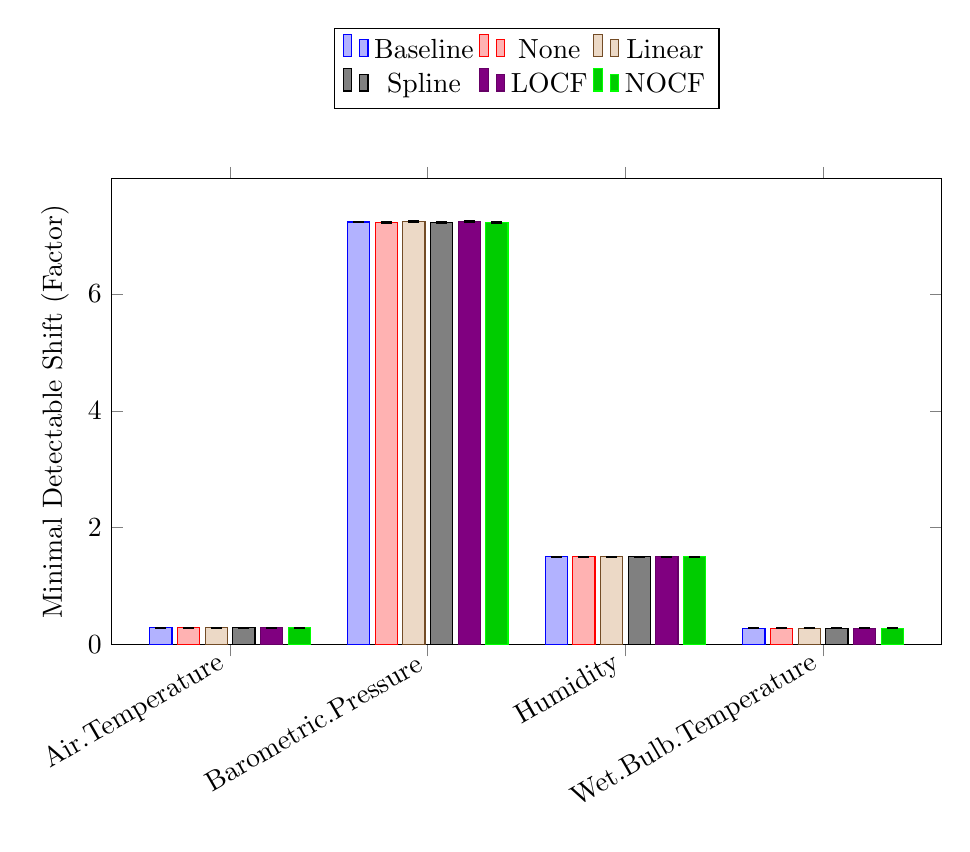
\begin{tikzpicture}
\begin{axis}[
    ybar,
    bar width=8pt,
    width=\textwidth,
    height=7.5cm,
    ymin=0,
    ylabel={Minimal Detectable Shift (Factor)},
    symbolic x coords={
        Air.Temperature,
        Barometric.Pressure,
        Humidity,
        Wet.Bulb.Temperature
    },
    xtick=data,
    x tick label style={rotate=30, anchor=east},
    enlarge x limits=0.2,
    legend style={
        at={(0.5,1.15)},
        anchor=south,
        legend columns=3
    },
    % Global error bar configuration (Corrected)
    error bars/y dir=both,
    error bars/y explicit,
    error bars/error bar style={line width=0.7pt, black},
    error bars/error mark options={
        rotate=90,
        mark size=2pt,
        line width=0.7pt
    }
]

% Baseline
\addplot coordinates {
    (Air.Temperature,0.2889756) +- (0,0.000136)
    (Barometric.Pressure,7.2321963) +- (0,0.006369)
    (Humidity,1.50479) +- (0,0.000805)
    (Wet.Bulb.Temperature,0.2770576) +- (0,0.000135)
};

% None
\addplot coordinates {
    (Air.Temperature,0.2891963) +- (0,0.000142)
    (Barometric.Pressure,7.2233516) +- (0,0.006437)
    (Humidity,1.5049092) +- (0,0.000827)
    (Wet.Bulb.Temperature,0.2772539) +- (0,0.000139)
};

% Linear
\addplot coordinates {
    (Air.Temperature,0.2889648) +- (0,0.000136)
    (Barometric.Pressure,7.2434307) +- (0,0.006195)
    (Humidity,1.502209) +- (0,0.000780)
    (Wet.Bulb.Temperature,0.2770947) +- (0,0.000141)
};

% Spline
\addplot coordinates {
    (Air.Temperature,0.2889512) +- (0,0.000140)
    (Barometric.Pressure,7.2291777) +- (0,0.006364)
    (Humidity,1.5026709) +- (0,0.000794)
    (Wet.Bulb.Temperature,0.2768818) +- (0,0.000143)
};

% LOCF
\addplot coordinates {
    (Air.Temperature,0.2889307) +- (0,0.000133)
    (Barometric.Pressure,7.2390908) +- (0,0.006329)
    (Humidity,1.5026436) +- (0,0.000782)
    (Wet.Bulb.Temperature,0.2770195) +- (0,0.000137)
};

% NOCF
\addplot coordinates {
    (Air.Temperature,0.2890967) +- (0,0.000140)
    (Barometric.Pressure,7.2291885) +- (0,0.006607)
    (Humidity,1.503333) +- (0,0.000784)
    (Wet.Bulb.Temperature,0.2771113) +- (0,0.000140)
};


\legend{Baseline, None, Linear, Spline, LOCF, NOCF}

\end{axis}
\end{tikzpicture}
\end{figure}


\begin{table}[htbp]
\centering
\caption{Minimal detectable shift with standard deviation under 10\% missingness.}
\label{tab:arl1_10pct}
\resizebox{\textwidth}{!}{%
\begin{tabular}{lcccccccccccc}
\toprule
& \multicolumn{2}{c}{Baseline}
& \multicolumn{2}{c}{None}
& \multicolumn{2}{c}{Linear}
& \multicolumn{2}{c}{Spline}
& \multicolumn{2}{c}{LOCF}
& \multicolumn{2}{c}{NOCF} \\
\cmidrule(lr){2-3}
\cmidrule(lr){4-5}
\cmidrule(lr){6-7}
\cmidrule(lr){8-9}
\cmidrule(lr){10-11}
\cmidrule(lr){12-13}
\textbf{Dataset}
& \textbf{Factor} & \textbf{SD}
& \textbf{Factor} & \textbf{SD}
& \textbf{Factor} & \textbf{SD}
& \textbf{Factor} & \textbf{SD}
& \textbf{Factor} & \textbf{SD}
& \textbf{Factor} & \textbf{SD}\\
\midrule
Air.Temperature & 0.2889756 & 0.004312669 & 0.2891963 & 0.004499342 & 0.2889648 & 0.004292358 & 0.2889512 & 0.004423248 & 0.2889307 & 0.00419322 & 0.2890967 & 0.004417068 \\
Barometric.Pressure     & 7.2321963 & 0.201267954 & 7.2233516 & 0.203409845 & 7.2434307 & 0.195779364 & 7.2291777 & 0.20108431 & 7.2390908 & 0.199938061 & 7.2291885 & 0.208750146 \\
Humidity     & 1.50479 & 0.025424252 & 1.5049092 & 0.026131511 & 1.502209 & 0.024633422 & 1.5026709 & 0.025088284 & 1.5026436 & 0.024699249 & 1.503333 & 0.024771174 \\
Wet.Bulb.Temperature & 0.2770576 & 0.004275104 & 0.2772539 & 0.004390379 & 0.2770947 & 0.00444939 & 0.2768818 & 0.004525685 & 0.2770195 & 0.004339007 & 0.2771113 & 0.004413131 \\
\bottomrule
\end{tabular}}
\end{table}

Across all interpolation strategies, minimal detectable shifts remain within 1–2\% of baseline values, even at elevated missingness. The observed stability of minimal detectable shifts falls within the expected statistical uncertainty, confirming that detection sensitivity is not materially affected by missingness.

\subsubsection{Minimal Detectable Shift Under 25\% Missingness}

Table~\ref{tab:arl1_25pct} reports detection performance under 25\% missingness.

\begin{figure}[htbp]
\centering
\caption{Minimal detectable shift with standard error under 25\% missingness for different imputation methods.}
\label{fig:arl1_25pct}

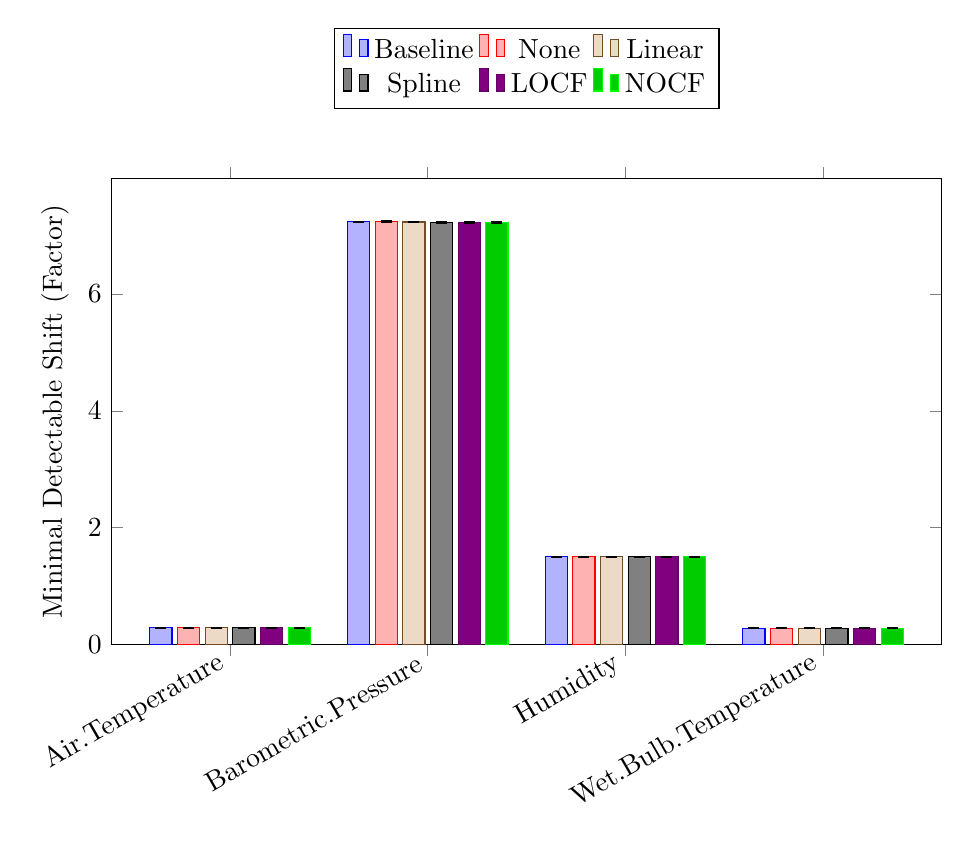
\begin{tikzpicture}
\begin{axis}[
    ybar,
    bar width=8pt,
    width=\textwidth,
    height=7.5cm,
    ymin=0,
    ylabel={Minimal Detectable Shift (Factor)},
    symbolic x coords={
        Air.Temperature,
        Barometric.Pressure,
        Humidity,
        Wet.Bulb.Temperature
    },
    xtick=data,
    x tick label style={rotate=30, anchor=east},
    enlarge x limits=0.2,
    legend style={
        at={(0.5,1.15)},
        anchor=south,
        legend columns=3
    },
    % Corrected global error bar settings
    error bars/y dir=both,
    error bars/y explicit,
    error bars/error bar style={line width=0.7pt, black},
    error bars/error mark options={
        rotate=90,
        mark size=2pt,
        line width=0.7pt
    }
]

% Baseline
\addplot coordinates {
    (Air.Temperature,0.2889756) +- (0,0.000136)
    (Barometric.Pressure,7.2321963) +- (0,0.006369)
    (Humidity,1.50479) +- (0,0.000805)
    (Wet.Bulb.Temperature,0.2770576) +- (0,0.000135)
};

% None
\addplot coordinates {
    (Air.Temperature,0.2889502) +- (0,0.000141)
    (Barometric.Pressure,7.2412695) +- (0,0.006272)
    (Humidity,1.5028398) +- (0,0.000753)
    (Wet.Bulb.Temperature,0.2770791) +- (0,0.000144)
};

% Linear
\addplot coordinates {
    (Air.Temperature,0.2887578) +- (0,0.000145)
    (Barometric.Pressure,7.2309629) +- (0,0.006131)
    (Humidity,1.5025977) +- (0,0.000781)
    (Wet.Bulb.Temperature,0.276877) +- (0,0.000145)
};

% Spline
\addplot coordinates {
    (Air.Temperature,0.2888174) +- (0,0.000143)
    (Barometric.Pressure,7.218416) +- (0,0.006343)
    (Humidity,1.5021787) +- (0,0.000757)
    (Wet.Bulb.Temperature,0.2769912) +- (0,0.000142)
};

% LOCF
\addplot coordinates {
    (Air.Temperature,0.2889004) +- (0,0.000142)
    (Barometric.Pressure,7.2240205) +- (0,0.006518)
    (Humidity,1.5025186) +- (0,0.000762)
    (Wet.Bulb.Temperature,0.2769414) +- (0,0.000138)
};

% NOCF
\addplot coordinates {
    (Air.Temperature,0.2889189) +- (0,0.000140)
    (Barometric.Pressure,7.219166) +- (0,0.006595)
    (Humidity,1.5030293) +- (0,0.000762)
    (Wet.Bulb.Temperature,0.2770381) +- (0,0.000137)
};

\legend{Baseline, None, Linear, Spline, LOCF, NOCF}

\end{axis}
\end{tikzpicture}
\end{figure}


\begin{table}[htbp]
\centering
\caption{Minimal detectable shift with standard deviation under 25\% missingness.}
\label{tab:arl1_25pct}
\resizebox{\textwidth}{!}{%
\begin{tabular}{lcccccccccccc}
\toprule
& \multicolumn{2}{c}{Baseline}
& \multicolumn{2}{c}{None}
& \multicolumn{2}{c}{Linear}
& \multicolumn{2}{c}{Spline}
& \multicolumn{2}{c}{LOCF}
& \multicolumn{2}{c}{NOCF} \\
\cmidrule(lr){2-3}
\cmidrule(lr){4-5}
\cmidrule(lr){6-7}
\cmidrule(lr){8-9}
\cmidrule(lr){10-11}
\cmidrule(lr){12-13}
\textbf{Dataset}
& \textbf{Factor} & \textbf{SD}
& \textbf{Factor} & \textbf{SD}
& \textbf{Factor} & \textbf{SD}
& \textbf{Factor} & \textbf{SD}
& \textbf{Factor} & \textbf{SD}
& \textbf{Factor} & \textbf{SD}\\
\midrule
Air.Temperature & 0.2889756 & 0.004312669 & 0.2889502 & 0.004447866 & 0.2887578 & 0.004585135 & 0.2888174 & 0.004505678 & 0.2889004 & 0.004495332 & 0.2889189 & 0.004412269 \\
Barometric.Pressure     & 7.2321963 & 0.201267954 & 7.2412695 & 0.198070084 & 7.2309629 & 0.193743069 & 7.218416 & 0.200414791 & 7.2240205 & 0.205989252 & 7.219166 & 0.208367355 \\
Humidity     & 1.50479 & 0.025424252 & 1.5028398 & 0.023779657 & 1.5025977 & 0.024673442 & 1.5021787 & 0.023935712 & 1.5025186 & 0.024081957 & 1.5030293 & 0.024088613 \\
Wet.Bulb.Temperature & 0.2770576 & 0.004275104 & 0.2770791 & 0.004557036 & 0.276877 & 0.004579183 & 0.2769912 & 0.004496843 & 0.2769414 & 0.004354214 & 0.2770381 & 0.004339365 \\
\bottomrule
\end{tabular}}
\end{table}

\subsubsection{Minimal Detectable Shift Under 50\% Missingness}

Table~\ref{tab:arl1_50pct} reports detection performance under 50\% missingness.

\begin{figure}[htbp]
\centering
\caption{Minimal detectable shift with standard error under 50\% missingness for different imputation methods.}
\label{fig:arl1_50pct}

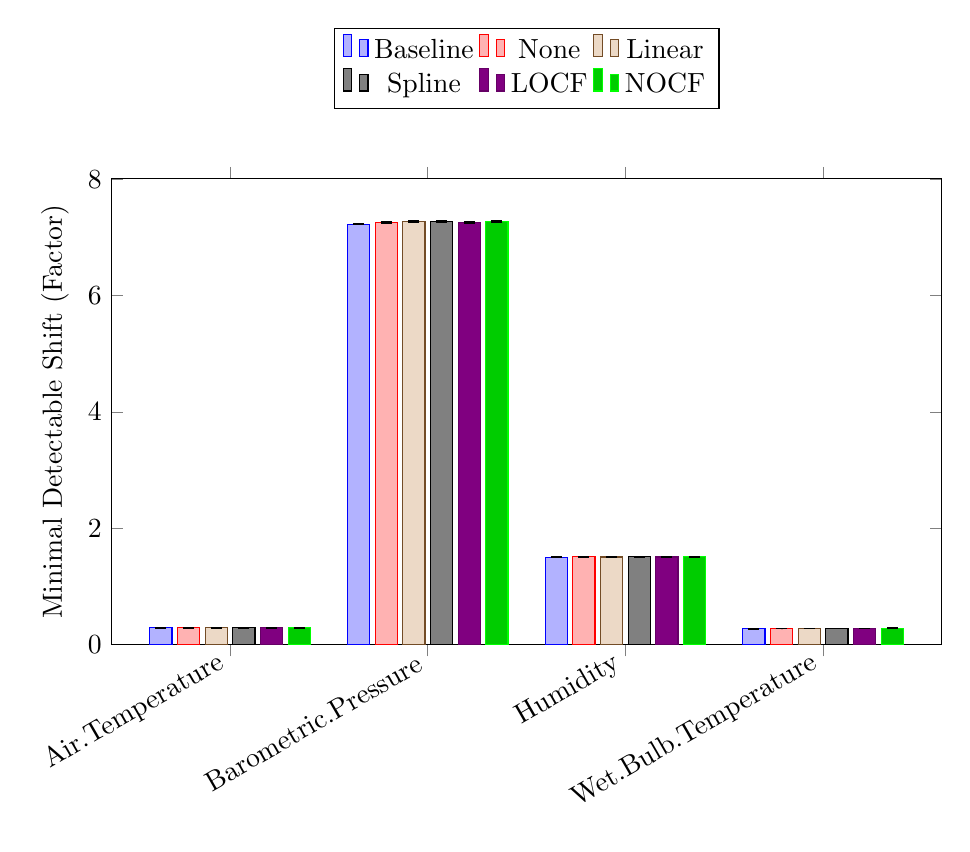
\begin{tikzpicture}
\begin{axis}[
    ybar,
    bar width=8pt,
    width=\textwidth,
    height=7.5cm,
    ymin=0,
    ylabel={Minimal Detectable Shift (Factor)},
    symbolic x coords={
        Air.Temperature,
        Barometric.Pressure,
        Humidity,
        Wet.Bulb.Temperature
    },
    xtick=data,
    x tick label style={rotate=30, anchor=east},
    enlarge x limits=0.2,
    legend style={
        at={(0.5,1.15)},
        anchor=south,
        legend columns=3
    },
    % Global error bar configuration
    error bars/y dir=both,
    error bars/y explicit,
    error bars/error bar style={line width=0.7pt, black},
    error bars/error mark options={
        rotate=90,
        mark size=2pt,
        line width=0.7pt
    }
]

% Baseline
\addplot coordinates {
    (Air.Temperature,0.2889756) +- (0,0.000136)
    (Barometric.Pressure,7.2321963) +- (0,0.006369)
    (Humidity,1.50479) +- (0,0.000805)
    (Wet.Bulb.Temperature,0.2770576) +- (0,0.000135)
};

% None
\addplot coordinates {
    (Air.Temperature,0.289083) +- (0,0.000162)
    (Barometric.Pressure,7.2634307) +- (0,0.006555)
    (Humidity,1.5085527) +- (0,0.000894)
    (Wet.Bulb.Temperature,0.2776729) +- (0,0.000158)
};

% Linear
\addplot coordinates {
    (Air.Temperature,0.2891992) +- (0,0.000162)
    (Barometric.Pressure,7.2790195) +- (0,0.006340)
    (Humidity,1.507208) +- (0,0.000912)
    (Wet.Bulb.Temperature,0.2776963) +- (0,0.000160)
};

% Spline
\addplot coordinates {
    (Air.Temperature,0.2895928) +- (0,0.000155)
    (Barometric.Pressure,7.2742275) +- (0,0.006497)
    (Humidity,1.5095664) +- (0,0.000880)
    (Wet.Bulb.Temperature,0.2780117) +- (0,0.000154)
};

% LOCF
\addplot coordinates {
    (Air.Temperature,0.2894561) +- (0,0.000155)
    (Barometric.Pressure,7.2613896) +- (0,0.006822)
    (Humidity,1.5076699) +- (0,0.000835)
    (Wet.Bulb.Temperature,0.2777334) +- (0,0.000153)
};

% NOCF
\addplot coordinates {
    (Air.Temperature,0.2896963) +- (0,0.000158)
    (Barometric.Pressure,7.2766982) +- (0,0.006338)
    (Humidity,1.5101016) +- (0,0.000914)
    (Wet.Bulb.Temperature,0.2781865) +- (0,0.000158)
};

\legend{Baseline, None, Linear, Spline, LOCF, NOCF}

\end{axis}
\end{tikzpicture}
\end{figure}


\begin{table}[htbp]
\centering
\caption{Minimal detectable shift with standard deviation under 50\% missingness.}
\label{tab:arl1_50pct}
\resizebox{\textwidth}{!}{%
\begin{tabular}{lcccccccccccc}
\toprule
& \multicolumn{2}{c}{Baseline}
& \multicolumn{2}{c}{None}
& \multicolumn{2}{c}{Linear}
& \multicolumn{2}{c}{Spline}
& \multicolumn{2}{c}{LOCF}
& \multicolumn{2}{c}{NOCF} \\
\cmidrule(lr){2-3}
\cmidrule(lr){4-5}
\cmidrule(lr){6-7}
\cmidrule(lr){8-9}
\cmidrule(lr){10-11}
\cmidrule(lr){12-13}
\textbf{Dataset}
& \textbf{Factor} & \textbf{SD}
& \textbf{Factor} & \textbf{SD}
& \textbf{Factor} & \textbf{SD}
& \textbf{Factor} & \textbf{SD}
& \textbf{Factor} & \textbf{SD}
& \textbf{Factor} & \textbf{SD}\\
\midrule
Air.Temperature & 0.2889756 & 0.004312669 & 0.289083 & 0.00512077 & 0.2891992 & 0.005110118 & 0.2895928 & 0.004907691 & 0.2894561 & 0.004893319 & 0.2896963 & 0.004943512 \\
Barometric.Pressure     & 7.2321963 & 0.201267954 & 7.2634307 & 0.207136903 & 7.2790195 & 0.200336268 & 7.2742275 & 0.205335137 & 7.2613896 & 0.215555379 & 7.2766982 & 0.200270948 \\
Humidity     & 1.50479 & 0.025424252 & 1.5085527 & 0.028234774 & 1.507208 & 0.028802067 & 1.5095664 & 0.027801018	 & 1.5076699 & 0.026374422 & 1.5101016 & 0.028876278 \\
Wet.Bulb.Temperature & 0.2770576 & 0.004275104 & 0.2776729 & 0.005006987 & 0.2776963 & 0.005061151 & 0.2780117 & 0.004880382 & 0.2777334 & 0.004845996 & 0.2781865 & 0.004993126 \\
\bottomrule
\end{tabular}}
\end{table}

\subsection{Detection Performance and Minimal Detectable Shift}

Minimal detectable shift factors remain relatively stable across missingness levels and interpolation methods, even at 50\% missingness. This indicates that interpolation preserves mean shift sensitivity reasonably well. This stability should not be interpreted as improved monitoring performance, as it often coincides with degraded \ac{ARL}$_0$.

However, this stability must not be interpreted as improved monitoring performance. In many configurations, stable shift detectability coincides with degraded \ac{ARL}$_0$, implying reduced reliability rather than increased sensitivity. In such cases, the chart signals more readily not because shifts are easier to detect, but because false alarms occur more frequently.

Thus, stable detection thresholds under missingness primarily reflect increased false-alarm activity rather than preserved statistical power.

% -----------------------------------------------------------------------
% Research Question 3:
% Influence of Extended reference timeframe on Missing Data on ARL_0
% -----------------------------------------------------------------------

\subsection{Effect of Extended Reference Timeframe}

\subsubsection{\ac{ARL}$_0$ Performance with Seasonal Extension}

Table~\ref{tab:arl0_missing_ext} compares \ac{ARL}$_0$ performance between standard and seasonally extended reference windows across all missingness levels.

\begin{figure}[htbp]
\centering
\caption{ARL$_0$ performance with standard error under missingness relative to baseline with extended reference timeframe}
\label{fig:arl0_missing_ext}

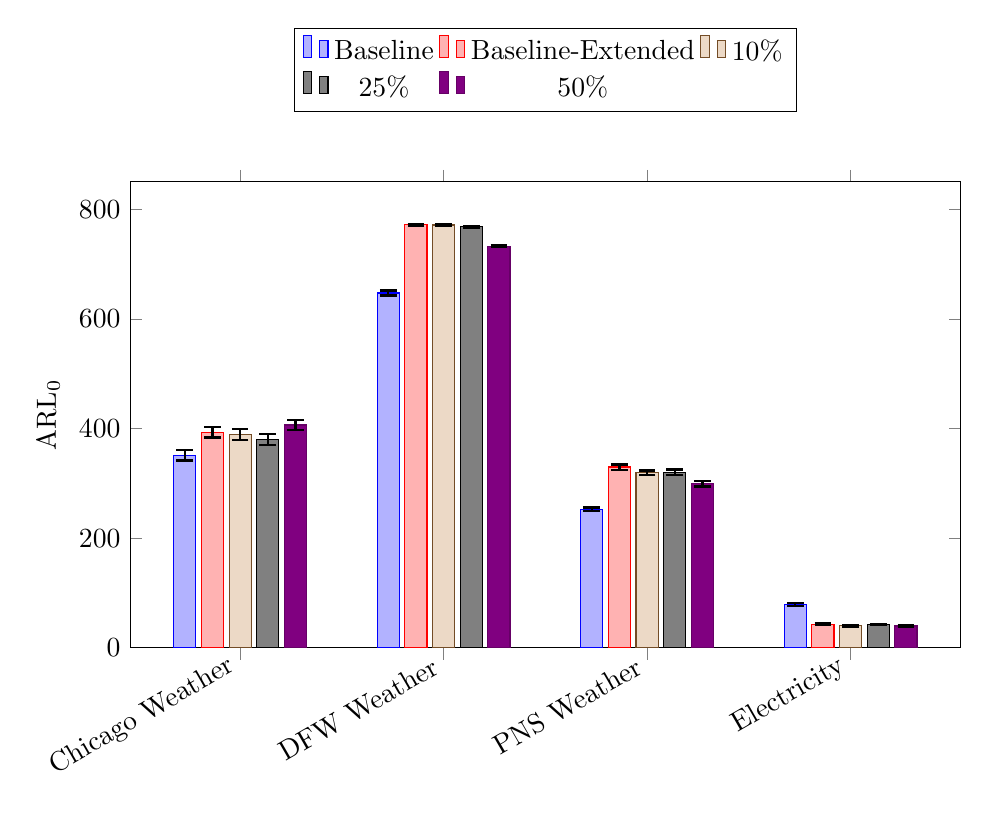
\begin{tikzpicture}
\begin{axis}[
    ybar,
    bar width=8pt, % Slightly reduced to accommodate 5 bars per group
    width=\textwidth,
    height=7.5cm,
    ymin=0,
    ylabel={ARL$_0$},
    symbolic x coords={
        Chicago Weather,
        DFW Weather,
        PNS Weather,
        Electricity
    },
    xtick=data,
    x tick label style={rotate=30, anchor=east},
    enlarge x limits=0.18,
    legend style={
        at={(0.5,1.15)},
        anchor=south,
        legend columns=3 % Better for 5 items (2 rows: 3 and 2)
    },
    % Global error bar configuration
    error bars/y dir=both,
    error bars/y explicit,
    error bars/error bar style={line width=0.8pt, black},
    error bars/error mark options={
        rotate=90,
        mark size=3pt,
        line width=0.8pt
    }
]

% Baseline
\addplot coordinates {
    (Chicago Weather,351.15) +- (0,9.414)
    (DFW Weather,647.166)   +- (0,4.672)
    (PNS Weather,252.783)   +- (0,2.872)
    (Electricity,78.979) +- (0,2.653)
};

% Baseline-Extended
\addplot coordinates {
    (Chicago Weather,393.127) +- (0,9.805)
    (DFW Weather,771.304)   +- (0,1.572)
    (PNS Weather,329.626)   +- (0,4.775)
    (Electricity,42.86) +- (0,1.520)
};

% 10%
\addplot coordinates {
    (Chicago Weather,388.66) +- (0,9.832)
    (DFW Weather,771.227)   +- (0,1.646)
    (PNS Weather,318.896)   +- (0,4.394)
    (Electricity,39.772) +- (0,1.393)
};

% 25%
\addplot coordinates {
    (Chicago Weather,380.068) +- (0,9.739)
    (DFW Weather,768.251)   +- (0,1.805)
    (PNS Weather,320.238)   +- (0,4.798)
    (Electricity,42.344) +- (0,1.503)
};

% 50%
\addplot coordinates {
    (Chicago Weather,406.264) +- (0,9.443)
    (DFW Weather,732.018)   +- (0,1.680)
    (PNS Weather,299.06)    +- (0,4.912)
    (Electricity,39.644) +- (0,1.451)
};

\legend{Baseline, Baseline-Extended, 10\%, 25\%, 50\%}

\end{axis}
\end{tikzpicture}
\end{figure}

Seasonal reference extension improves covariance estimation by increasing sample size and stabilizing marginal distributions across seasonal regimes.
For Electricity, reference extension fails to improve \ac{ARL}$_0$ due to persistent structural nonstationarity.

Reference extension is therefore beneficial for quasi-stationary environmental processes, but ineffective for load-driven systems.


\begin{table}[htbp]
\centering
\caption{ARL$_0$ performance with standard deviation under missingness relative to baseline with extended reference timeframe}
\label{tab:arl0_missing_ext}
\resizebox{\textwidth}{!}{%
\begin{tabular}{lcccccccccc}
\toprule
& \multicolumn{2}{c}{Baseline}
& \multicolumn{2}{c}{Baseline-Extended}
& \multicolumn{2}{c}{10\%}
& \multicolumn{2}{c}{25\%}
& \multicolumn{2}{c}{50\%} \\
\cmidrule(lr){2-3}
\cmidrule(lr){4-5}
\cmidrule(lr){6-7}
\cmidrule(lr){8-9}
\cmidrule(lr){10-11}
\textbf{Dataset}
& \textbf{ARL$_0$} & \textbf{SD}
& \textbf{ARL$_0$} & \textbf{SD}
& \textbf{ARL$_0$} & \textbf{SD}
& \textbf{ARL$_0$} & \textbf{SD}
& \textbf{ARL$_0$} & \textbf{SD} \\
\midrule
Chicago Weather & 351.15 & 297.3739948 & 393.127 & 309.8274163 & 388.66 & 310.7066446 & 380.068 & 307.6500934 & 406.264 & 298.3934902  \\
DFW Weather     & 647.166 & 147.6277087 & 771.304 & 49.68128233 & 771.227 & 52.01233271 & 768.251 & 57.03083829 & 732.018 & 53.08545697 \\
PNS Weather     & 252.783 & 90.75284012 & 329.626 & 150.9060395 & 318.896 & 138.8530207 & 320.238 & 151.6175889 & 299.06 & 155.1944126 \\
Electricity & 78.979 & 83.81632141 & 42.86 & 48.03961078 & 39.772 & 44.02272159 & 42.344 & 47.50164281 & 39.644 & 45.82304022 \\
\bottomrule
\end{tabular}}
\end{table}

\subsubsection{Summary of Seasonal Extension Effects}

Seasonal reference extension substantially improves \ac{ARL}$_0$ stability across all datasets. The effect is strongest for weather datasets, where seasonal dynamics dominate variability, and remains beneficial even under 50\% missingness.

Notably, the gains from reference extension exceed those obtained from interpolation alone, reinforcing the central claim of this thesis: robustness is primarily governed by reference construction rather than online data repair.


% -----------------------------------------------------------------------
% Research Question 4:
% Influence of Extended reference timeframe and imputation methods on Missing Data on ARL_0
% -----------------------------------------------------------------------

\subsection{Impact of Imputation on \ac{ARL}$_0$}

As described in previous chapters, the influence of four interpolation methods applied to the modified datasets with missing data has been assesed in regards to different degrees of missing data. The following subsections will show the results in regards to either 10\%, 25\%, or 50\%.

\subsubsection{10\% Missingness}

Table~\ref{tab:arl0_10pct_ext} presents \ac{ARL}$_0$ performance under 10\% random row deletion across different interpolation methods. 

\begin{figure}[htbp]
\centering
\caption{ARL$_0$ performance with standard error under 10\% missingness with extended reference timeframe for different imputation methods.}
\label{fig:arl0_10pct_ext}

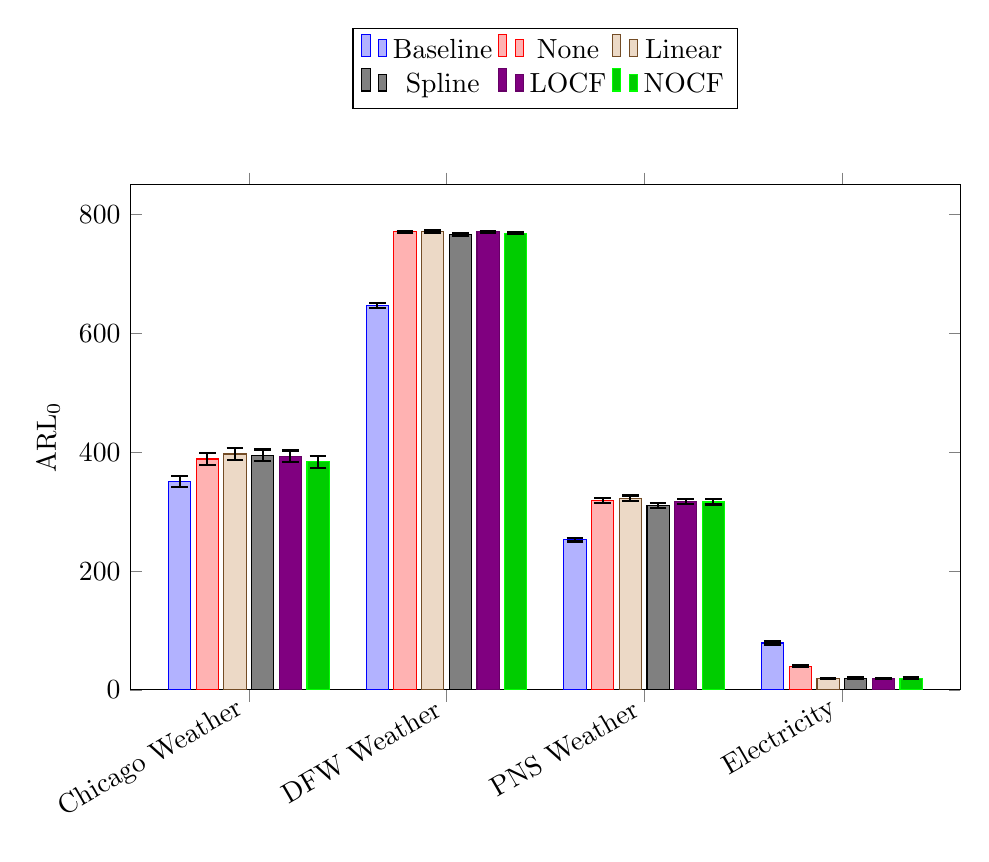
\begin{tikzpicture}
\begin{axis}[
    ybar,
    bar width=8pt, % Reduced to prevent bars from touching between categories
    width=\textwidth,
    height=8cm,
    ymin=0,
    ylabel={ARL$_0$},
    symbolic x coords={
        Chicago Weather,
        DFW Weather,
        PNS Weather,
        Electricity
    },
    xtick=data,
    x tick label style={rotate=30, anchor=east},
    enlarge x limits=0.2,
    legend style={
        at={(0.5,1.15)}, % Raised to avoid overlapping with high error bars
        anchor=south,
        legend columns=3 % Two neat rows of 3
    },
    % Corrected global error bar settings
    error bars/y dir=both,
    error bars/y explicit,
    error bars/error bar style={line width=0.8pt, black},
    error bars/error mark options={
        rotate=90,
        mark size=3pt,
        line width=0.8pt
    }
]

% Baseline
\addplot coordinates {
    (Chicago Weather,351.15) +- (0,9.414)
    (DFW Weather,647.166) +- (0,4.672)
    (PNS Weather,252.783) +- (0,2.872)
    (Electricity,78.979) +- (0,2.653)
};

% None
\addplot coordinates {
    (Chicago Weather,388.66) +- (0,9.832)
    (DFW Weather,771.227) +- (0,1.646)
    (PNS Weather,318.896) +- (0,4.394)
    (Electricity,39.772) +- (0,1.393)
};

% Linear
\addplot coordinates {
    (Chicago Weather,397.033) +- (0,9.866)
    (DFW Weather,771.632) +- (0,1.628)
    (PNS Weather,322.792) +- (0,4.309)
    (Electricity,19.576) +- (0,1.101)
};

% Spline
\addplot coordinates {
    (Chicago Weather,394.818) +- (0,9.835)
    (DFW Weather,766.846) +- (0,1.888)
    (PNS Weather,310.287) +- (0,4.314)
    (Electricity,19.706) +- (0,1.125)
};

% LOCF
\addplot coordinates {
    (Chicago Weather,393.157) +- (0,9.883)
    (DFW Weather,770.795) +- (0,1.749)
    (PNS Weather,317.519) +- (0,4.446)
    (Electricity,19.022) +- (0,1.047)
};

% NOCF
\addplot coordinates {
    (Chicago Weather,383.728) +- (0,9.731)
    (DFW Weather,768.772) +- (0,1.828)
    (PNS Weather,316.357) +- (0,4.329)
    (Electricity,19.841) +- (0,1.118)
};

\legend{Baseline, None, Linear, Spline, LOCF, NOCF}

\end{axis}
\end{tikzpicture}
\end{figure}


\begin{table}[htbp]
\centering
\caption{ARL$_0$ performance with standard deviation under 10\% missingness relative to baseline}
\label{tab:arl0_10pct_ext}
\resizebox{\textwidth}{!}{%
\begin{tabular}{lcccccccccccc}
\toprule
& \multicolumn{2}{c}{Baseline}
& \multicolumn{2}{c}{None}
& \multicolumn{2}{c}{Linear}
& \multicolumn{2}{c}{Spline}
& \multicolumn{2}{c}{LOCF}
& \multicolumn{2}{c}{NOCF} \\
\cmidrule(lr){2-3}
\cmidrule(lr){4-5}
\cmidrule(lr){6-7}
\cmidrule(lr){8-9}
\cmidrule(lr){10-11}
\cmidrule(lr){12-13}
\textbf{Dataset}
& \textbf{ARL$_0$} & \textbf{SD}
& \textbf{ARL$_0$} & \textbf{SD}
& \textbf{ARL$_0$} & \textbf{SD}
& \textbf{ARL$_0$} & \textbf{SD}
& \textbf{ARL$_0$} & \textbf{SD}
& \textbf{ARL$_0$} & \textbf{SD} \\
\midrule
Chicago Weather & 351.15 & 297.3739948 & 388.66 & 310.7066446 & 397.033 & 311.5507981 & 394.818 & 310.8683645 & 393.157 & 312.2944671 & 383.728 & 307.4908855 \\
DFW Weather     & 647.166 & 147.6277087 & 771.227 & 52.01233271 & 771.632 & 51.43360761 & 766.846 & 59.65538575 & 770.795 & 55.26884856 & 768.772 & 57.7450648 \\
PNS Weather     & 252.783 & 90.75284012 & 318.896 & 138.8530207 & 322.792 & 136.1585983 & 310.287 & 136.335586 & 317.519 & 140.4535255 & 316.357 & 136.8181741 \\
Electricity & 78.979 & 83.81632141 & 39.772 & 44.02272159 & 19.576 & 34.79797585 & 19.706 & 35.55246182 & 19.022 & 33.08589113  & 19.841 & 35.32287395 \\
\bottomrule
\end{tabular}}
\end{table}



\subsubsection{25\% Missingness}

Table~\ref{tab:arl0_25pct_ext} presents \ac{ARL}$_0$ performance under 25\% random row deletion.

\begin{figure}[htbp]
\centering
\caption{ARL$_0$ performance with standard error under 25\% missingness with extended reference timeframe for different imputation methods.}
\label{fig:arl0_25pct_ext}

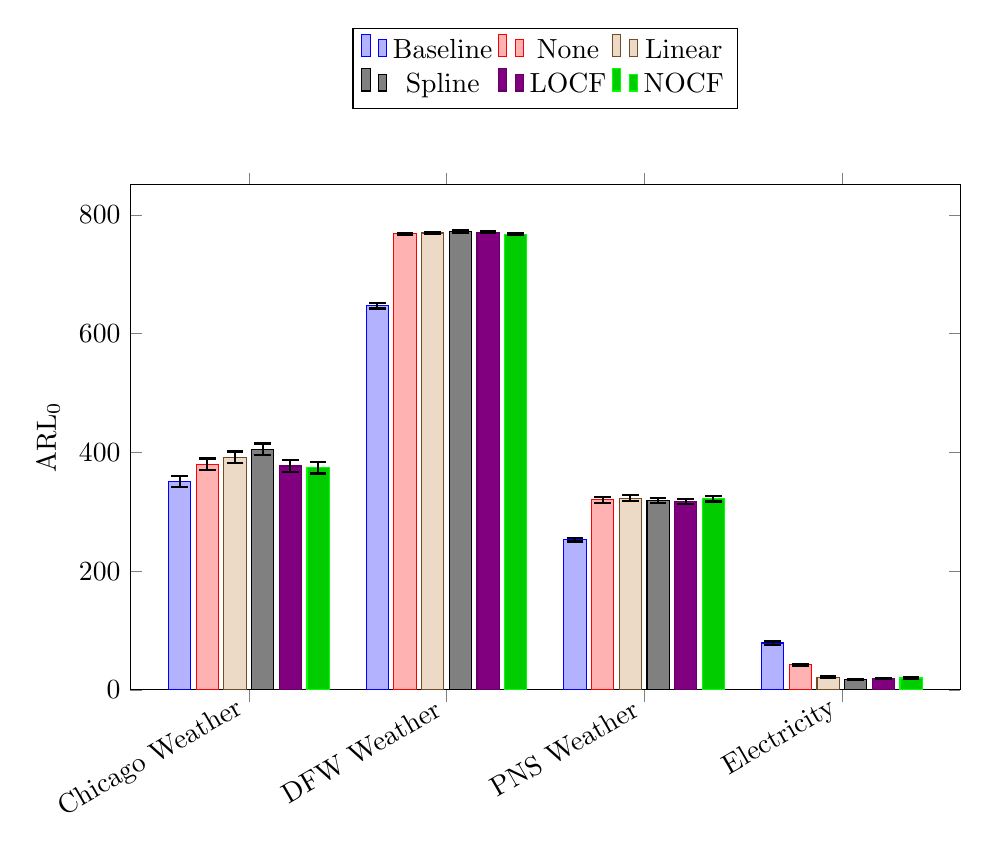
\begin{tikzpicture}
\begin{axis}[
    ybar,
    bar width=8pt,
    width=\textwidth,
    height=8cm,
    ymin=0,
    ylabel={ARL$_0$},
    symbolic x coords={
        Chicago Weather,
        DFW Weather,
        PNS Weather,
        Electricity
    },
    xtick=data,
    x tick label style={rotate=30, anchor=east},
    enlarge x limits=0.2,
    legend style={
        at={(0.5,1.15)},
        anchor=south,
        legend columns=3
    },
    % Corrected global error bar settings
    error bars/y dir=both,
    error bars/y explicit,
    error bars/error bar style={line width=0.8pt, black},
    error bars/error mark options={
        rotate=90,
        mark size=3pt,
        line width=0.8pt
    }
]

% Baseline
\addplot coordinates {
    (Chicago Weather,351.15) +- (0,9.414)
    (DFW Weather,647.166) +- (0,4.672)
    (PNS Weather,252.783) +- (0,2.872)
    (Electricity,78.979) +- (0,2.653)
};

% None
\addplot coordinates {
    (Chicago Weather,380.068) +- (0,9.739)
    (DFW Weather,768.251) +- (0,1.805)
    (PNS Weather,320.238) +- (0,4.798)
    (Electricity,42.344) +- (0,1.503)
};

% Linear
\addplot coordinates {
    (Chicago Weather,392.053) +- (0,9.803)
    (DFW Weather,769.843) +- (0,1.838)
    (PNS Weather,322.979) +- (0,4.809)
    (Electricity,21.67) +- (0,1.274)
};

% Spline
\addplot coordinates {
    (Chicago Weather,405.337) +- (0,9.886)
    (DFW Weather,772.335) +- (0,1.690)
    (PNS Weather,319.096) +- (0,4.602)
    (Electricity,17.93) +- (0,0.998)
};

% LOCF
\addplot coordinates {
    (Chicago Weather,377.197) +- (0,9.778)
    (DFW Weather,771.144) +- (0,1.733)
    (PNS Weather,317.68) +- (0,4.476)
    (Electricity,19.632) +- (0,1.103)
};

% NOCF
\addplot coordinates {
    (Chicago Weather,374.273) +- (0,9.747)
    (DFW Weather,767.663) +- (0,1.799)
    (PNS Weather,322.36) +- (0,4.833)
    (Electricity,20.077) +- (0,1.061)
};

\legend{Baseline, None, Linear, Spline, LOCF, NOCF}

\end{axis}
\end{tikzpicture}
\end{figure}



\begin{table}[htbp]
\centering
\caption{\ac{ARL}$_0$ performance with standard deviation under 25\% missingness.}
\label{tab:arl0_25pct_ext}
\resizebox{\textwidth}{!}{%
\begin{tabular}{lcccccccccccc}
\toprule
& \multicolumn{2}{c}{Baseline}
& \multicolumn{2}{c}{None}
& \multicolumn{2}{c}{Linear}
& \multicolumn{2}{c}{Spline}
& \multicolumn{2}{c}{LOCF}
& \multicolumn{2}{c}{NOCF} \\
\cmidrule(lr){2-3}
\cmidrule(lr){4-5}
\cmidrule(lr){6-7}
\cmidrule(lr){8-9}
\cmidrule(lr){10-11}
\cmidrule(lr){12-13}
\textbf{Dataset}
& \textbf{ARL$_0$} & \textbf{SD}
& \textbf{ARL$_0$} & \textbf{SD}
& \textbf{ARL$_0$} & \textbf{SD}
& \textbf{ARL$_0$} & \textbf{SD}
& \textbf{ARL$_0$} & \textbf{SD}
& \textbf{ARL$_0$} & \textbf{SD} \\
\midrule
Chicago Weather & 351.15 & 297.3739948 & 380.068 & 307.6500934 & 392.053 & 309.7007148 & 405.337 & 312.4373033 & 377.197 & 308.8738987 & 374.273 & 308.0035205 \\
DFW Weather     & 647.166 & 147.6277087 & 768.251 & 57.03083829 & 769.843	& 58.07718408 & 772.335 & 53.40935624	& 771.144 & 54.7774208 & 767.663 & 56.85817693 \\
PNS Weather     & 252.783 & 90.75284012 & 320.238 & 151.6175889 & 322.979 & 151.945062 & 319.096 & 145.397005 & 317.68 & 141.3939314 & 322.36 & 152.7370715 \\
Electricity & 78.979 & 83.81632141 & 42.344 & 47.50164281 & 21.67 & 40.27827503  & 17.93 & 31.53203719 & 19.632 & 34.8641088  & 20.077 & 33.52848386 \\
\bottomrule
\end{tabular}}
\end{table}

\subsubsection{50\% Missingness}

Table~\ref{tab:arl0_50pct_ext} presents \ac{ARL}$_0$ performance under 50\% random row deletion.

\begin{figure}[htbp]
\centering
\caption{ARL$_0$ performance with standard error under 50\% missingness with extended reference timeframe for different imputation methods.}
\label{fig:arl0_50pct_ext}

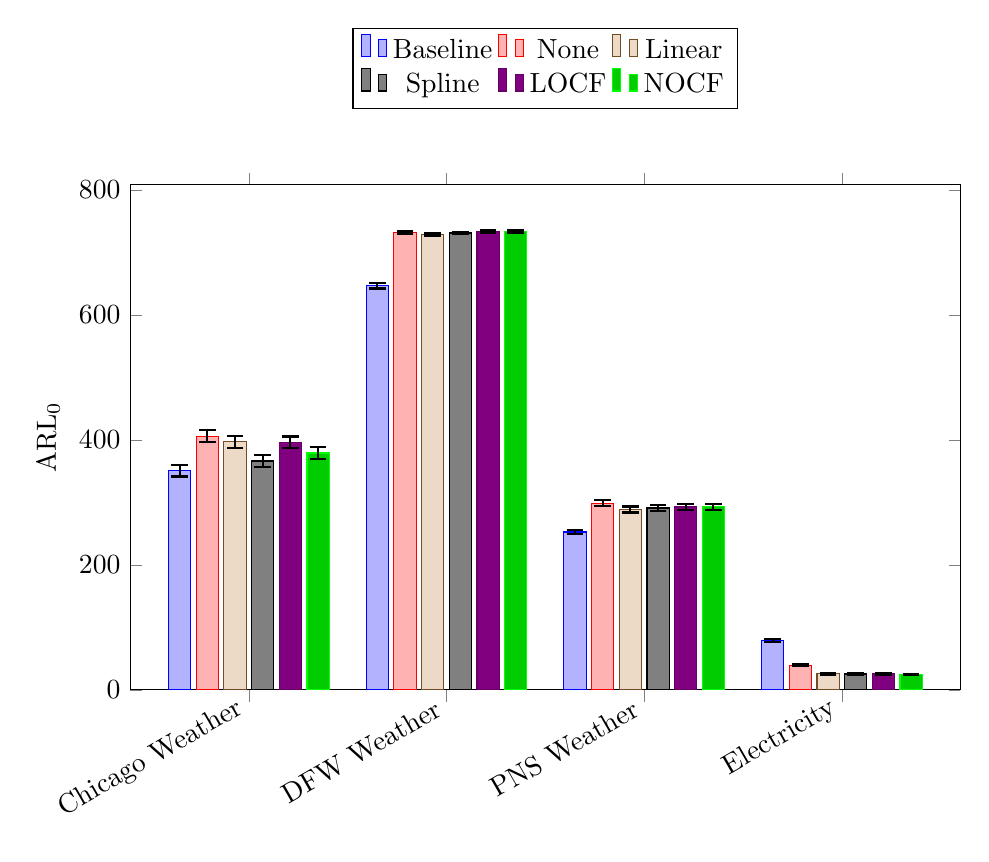
\begin{tikzpicture}
\begin{axis}[
    ybar,
    bar width=8pt,
    width=\textwidth,
    height=8cm,
    ymin=0,
    ylabel={ARL$_0$},
    symbolic x coords={
        Chicago Weather,
        DFW Weather,
        PNS Weather,
        Electricity
    },
    xtick=data,
    x tick label style={rotate=30, anchor=east},
    enlarge x limits=0.2,
    legend style={
        at={(0.5,1.15)},
        anchor=south,
        legend columns=3
    },
    % Corrected global error bar settings
    error bars/y dir=both,
    error bars/y explicit,
    error bars/error bar style={line width=0.8pt, black},
    error bars/error mark options={
        rotate=90,
        mark size=3pt,
        line width=0.8pt
    }
]

% Baseline
\addplot coordinates {
    (Chicago Weather,351.15) +- (0,9.414)
    (DFW Weather,647.166) +- (0,4.672)
    (PNS Weather,252.783) +- (0,2.872)
    (Electricity,78.979) +- (0,2.653)
};

% None
\addplot coordinates {
    (Chicago Weather,406.264) +- (0,9.443)
    (DFW Weather,732.018) +- (0,1.680)
    (PNS Weather,299.06) +- (0,4.912)
    (Electricity,39.644) +- (0,1.451)
};

% Linear
\addplot coordinates {
    (Chicago Weather,397.182) +- (0,9.467)
    (DFW Weather,728.53) +- (0,1.866)
    (PNS Weather,288.737) +- (0,4.683)
    (Electricity,25.675) +- (0,1.279)
};

% Spline
\addplot coordinates {
    (Chicago Weather,366.376) +- (0,9.382)
    (DFW Weather,731.254) +- (0,1.713)
    (PNS Weather,291.138) +- (0,4.717)
    (Electricity,25.514) +- (0,1.177)
};

% LOCF
\addplot coordinates {
    (Chicago Weather,396.247) +- (0,9.456)
    (DFW Weather,733.496) +- (0,1.652)
    (PNS Weather,292.784) +- (0,4.698)
    (Electricity,25.892) +- (0,1.311)
};

% NOCF
\addplot coordinates {
    (Chicago Weather,379.12) +- (0,9.414)
    (DFW Weather,733.528) +- (0,1.796)
    (PNS Weather,293.034) +- (0,4.748)
    (Electricity,24.923) +- (0,1.204)
};

\legend{Baseline, None, Linear, Spline, LOCF, NOCF}

\end{axis}
\end{tikzpicture}
\end{figure}


\begin{table}[htbp]
\centering
\caption{\ac{ARL}$_0$ performance with standard deviation under 50\% missingness.}
\label{tab:arl0_50pct_ext}
\resizebox{\textwidth}{!}{%
\begin{tabular}{lcccccccccccc}
\toprule
& \multicolumn{2}{c}{Baseline}
& \multicolumn{2}{c}{None}
& \multicolumn{2}{c}{Linear}
& \multicolumn{2}{c}{Spline}
& \multicolumn{2}{c}{LOCF}
& \multicolumn{2}{c}{NOCF} \\
\cmidrule(lr){2-3}
\cmidrule(lr){4-5}
\cmidrule(lr){6-7}
\cmidrule(lr){8-9}
\cmidrule(lr){10-11}
\cmidrule(lr){12-13}
\textbf{Dataset}
& \textbf{ARL$_0$} & \textbf{SD}
& \textbf{ARL$_0$} & \textbf{SD}
& \textbf{ARL$_0$} & \textbf{SD}
& \textbf{ARL$_0$} & \textbf{SD}
& \textbf{ARL$_0$} & \textbf{SD}
& \textbf{ARL$_0$} & \textbf{SD} \\
\midrule
Chicago Weather & 351.15 & 297.3739948 & 406.264 & 298.3934902 & 397.182 & 299.1356064 & 366.376 & 296.4089015 & 396.247 & 298.7183065 & 379.12 & 297.3940632 \\
DFW Weather     & 647.166 & 147.6277087 & 732.018 & 53.08545697 & 728.53 & 58.96077911 & 731.254 & 54.13991702 & 733.496 & 52.20831056 & 733.528 & 56.75269231 \\
PNS Weather     & 252.783 & 90.75284012 & 299.06 & 155.1944126 & 288.737 & 147.9167644 & 291.138 & 149.0095796 & 292.784 & 148.3663301 & 293.034 & 150.0635929 \\
Electricity & 78.979 & 83.81632141 & 39.644 & 45.82304022 & 25.675 & 40.40514758  & 25.514 & 37.16262726 & 25.892 & 41.43628001 & 24.923 & 38.06065796 \\
\bottomrule
\end{tabular}}
\end{table}


\subsection{Summary}

Taken together, these results demonstrate that interpolation primarily alters the temporal structure of the monitoring statistic rather than restoring its statistical properties. Differences in mean performance metrics generally remain within statistical uncertainty, while variability increases substantially under missingness. Apparent robustness is therefore largely illusory, driven by increased false-alarm activity rather than preserved detection power. In contrast, reference construction—particularly seasonal extension—provides a more effective mechanism for stabilizing monitoring behavior. These findings motivate the methodological recommendations discussed in Chapter~5.
